\subsection{53 cartes}

\renewcommand{\CURPATH}{examples/solitaire/53}

Maintenant, regardons la première partie de la boucle:

\begin{lstlisting}
.text:0000000100036684 loc_100036684:                          ; CODE XREF: SolitaireGame::InitialDeal(void)+C0↓j
.text:0000000100036684                 mov     eax, 4EC4EC4Fh
.text:0000000100036689                 mul     edi
.text:000000010003668B                 mov     r8d, edx
.text:000000010003668E                 shr     r8d, 4          ; unsigned int
.text:0000000100036692                 mov     eax, r8d
.text:0000000100036695                 imul    eax, 52
.text:0000000100036698                 mov     edx, edi
.text:000000010003669A                 sub     edx, eax        ; unsigned int
.text:000000010003669C                 mov     rcx, [rbx+128h] ; this
.text:00000001000366A3                 call    ?CreateCard@CardTable@@IEAAPEAVCard@@II@Z ; CardTable::CreateCard(uint,uint)
.text:00000001000366A8                 mov     rdx, rax        ; struct Card *
.text:00000001000366AB                 mov     rcx, rbx        ; this
.text:00000001000366AE                 call    ?Push@CardStack@@QEAAXPEAVCard@@@Z ; CardStack::Push(Card *)
.text:00000001000366B3                 inc     edi
.text:00000001000366B5                 cmp     edi, 52
.text:00000001000366B8                 jb      short loc_100036684
\end{lstlisting}

Qu'est-ce que cette multiplication par 4EC4EC4Fh? Il s'agit sûrement de la division
par la multiplication.
Et voici ce qu'Hex-Rays en dit:

\begin{lstlisting}
  v5 = 0;
  do
  {
    v6 = CardTable::CreateCard(v4[37], v5 % 0x34, v5 / 0x34);
    CardStack::Push((CardStack *)v4, v6);
    ++v5;
  }
  while ( v5 < 0x34 );
\end{lstlisting}

D'une certaine façon, la fonction \verb|CreateCard()| prend deux arguments:
l'itérateur divisé par 52 et le reste de l'opération de division.
Difficile de dire pourquoi ils ont fait ainsi.
Le Solitaire ne peut pas permettre plus de 52 cartes, donc le dernier argument
est absurde, il vaut toujours zéro.

Mais une fois que j'ai modifié l'instruction \TT{cmp edi, 52} en 0x1000366B5 par
\TT{cmp edi, 53}, j'ai trouvé qu'il y avait maintenant 53 cartes.
La dernière est le \textit{deux de trèfle}, car il s'agit de la carte numérotée
0.

Lors de la dernière itération, 0x52 est divisé par 0x52, le reste est zéro, donc
la carte d'indice 0 est ajoutée deux fois.

Que c'est frustrant, il y a deux \textit{deux de trèfle}:

\begin{figure}[H]
\centering
\frame{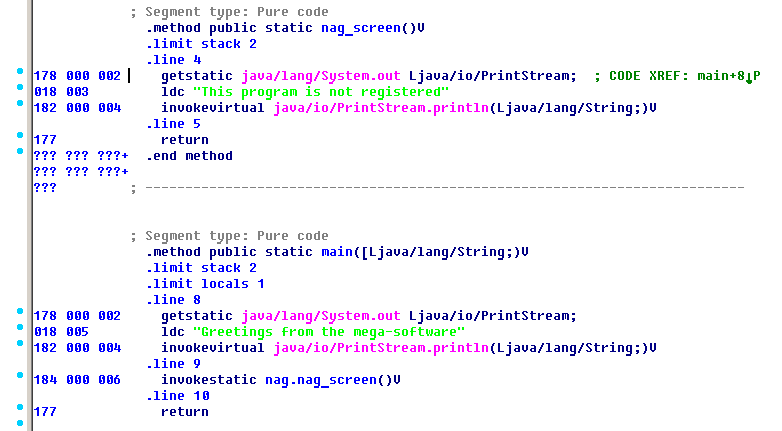
\includegraphics[width=\textwidth]{\CURPATH/1.png}}
\end{figure}

Ceci est le Solitaire de Windows 7 modifié:
\href{\RepoURL/examples/solitaire/53/Solitaire53.exe}{Solitaire53.exe}.

